\chapter{Nền tảng: Ngôn ngữ hệ thống cho phần mềm nhạy độ trễ\label{chapter:background}}
% The class prints the chapter titles in the running head in capitals, where the
% full title of this chapter runs into the margin.
\chaptermark{Nền tảng}

\section{Hệ thống mặt điều khiển RAN và gNB-CU-CP}\label{sec:ranarch}
Mạng truy nhập vô tuyến thế hệ mới (NG-RAN) là bối cảnh của phép so sánh này. Tốc độ sự kiện
cao: UE di chuyển, và báo hiệu có thể tăng đột biến. Giới hạn trễ chặt và phải ổn định. Các
đặc tả dịch vụ và RAN 5G nêu những giới hạn đó như chỉ số hiệu năng then chốt
(KPI)~\cite{3gpp38913,3gpp22261}. Phần mềm sống lâu và tiếp tục lớn. Nhiều luồng chạy cùng lúc.
Ở đây trường hợp xấu nhất và đuôi quan trọng hơn trung bình. Đó là lý do luận văn này đo đuôi.

gNB được tách theo hai trục. Tách thứ nhất là trung tâm đối với phân tán. Một đơn vị trung tâm
(gNB-CU) lưu các tầng cao hơn của ngăn xếp. Một hoặc nhiều đơn vị phân tán (gNB-DU) lưu các
tầng thấp hơn. Những tầng đó nằm gần vô tuyến và chặt về thời gian. Tách thứ hai là mặt điều
khiển đối với mặt người dùng, bên trong đơn vị trung tâm. Nó tách chức năng mặt điều khiển
(gNB-CU-CP) khỏi chức năng mặt người dùng (gNB-CU-UP). Các phần này nói chuyện qua liên kết
chuẩn. NG đi về lõi 5G. F1 nằm giữa CU và DU. E1 nằm giữa CU-CP và
CU-UP~\cite{3gpp38401,3gpp38300,3gpp38463}. Open-RAN đẩy cùng các liên kết đó xa hơn. Mỗi phần
khi đó có thể đến từ một nhà cung cấp khác và chạy như phần mềm trên máy thông
thường~\cite{polese2023oran}. Hình~\ref{fig:ngran} đặt phân hệ được nghiên cứu ở đây, Quản lý
Ngữ cảnh UE (UECM), bên trong gNB-CU-CP. UECM sở hữu trạng thái mặt điều khiển theo từng UE.
Nó cũng xử lý báo hiệu RRC và di động. Đó là lý do tính đúng đắn và thời gian của nó đứng cho
mặt điều khiển nói chung.

% After the two paragraphs the leftover is a few points short of the TikZ plus
% caption, so [ht] defers it and [section]{placeins} ships the leftover as
% whitespace. A small enlarge keeps the figure with the section that cites it.
\enlargethispage{12pt}
\begin{figure}[!ht]
\centering
\begin{tikzpicture}[
    font=\small, >={Stealth[length=2.4mm]},
    box/.style={draw, rounded corners, minimum height=1.0cm, minimum width=1.7cm,
                align=center, fill=gray!8},
    cpbox/.style={draw, rounded corners, align=center, fill=blue!8},
    upbox/.style={draw, rounded corners, minimum width=3.1cm, minimum height=0.8cm,
                  align=center, fill=green!8},
    uecm/.style={draw, rounded corners, minimum width=2.7cm, minimum height=0.62cm,
                 fill=red!14, align=center}
  ]
  \node[box] (ue) at (0,0)   {UE};
  \node[box] (du) at (2.4,0) {gNB-DU};

  \node[font=\footnotesize\bfseries] (cpttl) at (7.2,1.7) {gNB-CU-CP};
  \node[uecm] (uecm) at (7.2,0.85) {Quản lý ngữ cảnh\\ UE};
  \node[upbox] (up) at (7.2,-0.95) {gNB-CU-UP};

  \begin{scope}[on background layer]
    \node[fit=(cpttl)(uecm), inner sep=6pt] (cp) {};
    \node[draw, dashed, rounded corners, fill=gray!3,
          fit=(cp)(up), inner sep=10pt, label={[font=\footnotesize\bfseries]above:gNB-CU}] (cu) {};
    \node[cpbox, fit=(cp), inner sep=0pt] {};
  \end{scope}

  \node[box] (core) at (11.4,0) {Lõi 5G};

  \draw[<->] (ue) -- node[above,font=\scriptsize]{Uu} (du);
  \draw[<->] (du.east)         -- node[above,font=\scriptsize]{F1} (cu.west |- du);
  \draw[<->] (cu.east |- core) -- node[above,font=\scriptsize]{NG} (core.west);
  \draw[<->] (cp.south) -- node[right,font=\scriptsize]{E1} (up.north);
\end{tikzpicture}
\caption[Phân hệ nghiên cứu nằm ở đâu trong NG-RAN 5G]{Phân hệ nghiên cứu nằm ở đâu trong
NG-RAN 5G. Quản lý Ngữ cảnh UE được tô đậm bên trong gNB-CU-CP.\label{fig:ngran}}
\end{figure}

\section{Khả năng dự đoán và hai ngôn ngữ}\label{sec:bgbrief}
Mục này nêu những gì nghiên cứu lấy làm cho trước. Độ trễ ổn định, không phải thông lượng trung
bình, là thuộc tính chính của một dịch vụ nhạy trễ. Vì vậy đại lượng cần đo là đuôi, không phải
trung bình. Đo đuôi tốt cũng định hình khung đo. Lịch gửi phải là vòng hở. Một bộ gửi vòng kín
dừng khi một tắc đang diễn ra. Nó rồi không bao giờ ghi lại độ trễ của tắc đó.

C++ cho kiểm soát mà miền cần. Nó để an toàn bộ nhớ và luồng cho lập trình viên. Bộ dò lỗi và
rà soát đứng thay cho một bảo đảm. Công việc của uỷ ban chuẩn về hồ sơ an toàn được thực thi
chưa phải một chuẩn. Nó chưa được dùng rộng. Sở hữu và mượn của Rust loại lỗi vòng đời và
aliasing tại thời điểm biên dịch. Các trait \texttt{Send} và \texttt{Sync} loại tranh chấp dữ
liệu. Tuyên bố đó hẹp hơn ``an toàn luồng''. Nó không nói gì về thứ tự khoá. Nó không nói gì về
việc một bước ghép có nguyên tử hay không. Nó không nói gì về rò rỉ. Và nó tắt ở mọi nơi chương
trình viết \texttt{unsafe}. Cả hai ngôn ngữ đều diễn đạt được cùng cấu trúc luồng. Một phép so
sánh để cấu trúc đổi theo ngôn ngữ khi đó đo cấu trúc, không đo ngôn ngữ. Hai bên gặp nhau qua
một giao diện nhị phân ứng dụng C. Đó là đường mà mọi di trú từng bước phải dùng. Đó cũng là
lý do một đường nối giữ \texttt{unsafe} mà một cuộc di trú cần.

\section{Khoảng trống nghiên cứu}\label{sec:gap}
Các mục trên dựng khoảng trống. Mặt điều khiển RAN có nhiều luồng và giới hạn trễ chặt. Độ trễ
đuôi khi tải quá lớn, không phải thông lượng trung bình, đặt chất lượng mà mạng giao. C++ cho
kiểm soát và tốc độ mà miền cần. Nhưng nó để cả lớp lỗi bộ nhớ và luồng cho phát hiện sau. Rust
hứa chặn những lớp đó tại thời điểm biên dịch mà không tốn thời gian chạy. Nó cũng cho một
đường áp dụng từng bước qua giao diện nhị phân ứng dụng (ABI) C.

Miền này không phải chưa được nghiên cứu. Khối lượng công trình trước dễ bị bỏ sót, vì gần như
không công trình nào được lập chỉ mục. Năm luận văn thạc sĩ do nhà cung cấp lưu trữ, tất cả
thực hiện tại Ericsson, đã so sánh các ngôn ngữ ứng viên cho phần mềm RAN và viễn thông. Một
bài cân chi phí lúc chạy với tốc độ con người xây được, trên C++, Rust và
Go~\cite{karlback2021ran}. Một bài hỏi liệu Rust có thể thay C trong quản lý nút
RAN~\cite{olsson2023ranmgmt}. Một bài xây bộ xử lý gói, một luồng mỗi nhân, bằng Rust async. Nó
đo bộ xử lý đó đối với chương trình Data Plane Development Kit (DPDK) mà nó
nhái~\cite{olsson2023asyncpackets}. Một bài đo độ trễ trung vị và p99 cho các bước mặt điều
khiển trên năm khung async~\cite{arvidsson2025async}. Bài cuối xây các bản C++ và Rust khớp
nhau của một bộ dịch ngược Abstract Syntax Notation One (ASN.1). Nó so sánh chúng bằng kiểm
định thống kê~\cite{emberg2023asn1}. Cả năm đều liên quan trực tiếp. Hai bài báo cáo khoảng
cách không nghiêng về Rust.

Ba trong số đó đổi ngôn ngữ cùng lúc với thời gian chạy và mô hình luồng. Một khoảng cách đo
được khi đó không thể quy cho ngôn ngữ chứ không phải khung~\cite{karlback2021ran,olsson2023asyncpackets,arvidsson2025async}.
Cỡ hiệu ứng lên tới hệ số năm. Điều đó cho thấy thời gian chạy chiếm bao nhiêu của phép đo. Hai
bài kia giữ thiết kế sát hơn với cố định. Nhưng chúng báo cáo thời gian chạy và bộ nhớ đỉnh,
không phải độ trễ đuôi dưới tải tăng~\cite{olsson2023ranmgmt,emberg2023asn1}. Bài gần nhất,
Emberg và Wadsten, đo một phép biến đổi không trạng thái. Nó không phải một phần nhiều luồng
có trạng thái. Hình~\ref{fig:gapmap} đặt năm luận văn nhà cung cấp cạnh các so sánh đa mục
đích~\cite{pereira2017energy} và các cặp phần mềm hệ thống khớp~\cite{emmerich2019drivers,suchert2023stamp}.
Mẫu hình như sau. Mỗi nhóm giữ một phần những gì một phép thử công bằng cần. Không nhóm nào giữ
hết.

Sự tập trung đó tự nó là một phần của khoảng trống. Cả năm nghiên cứu đến từ một nhà cung cấp.
Kết luận của chúng chưa bao giờ được thử đối với phần mềm, mục tiêu hay quy tắc nội bộ của một
công ty khác. Vì vậy những gì được biết về câu hỏi này là những gì khung của một công ty nói về
nó. Hồ sơ công bố phía bên kia mỏng hơn. Không có nghiên cứu về Rust trong các bài được lập chỉ
mục của nhà cung cấp chủ trì công trình này. Lập trường đã bình duyệt gần nhất từ phía đó lập
luận cho việc làm vệ sinh lỗi bộ nhớ trở nên thực tế. Nó không lập luận thay vệ sinh đó bằng
một bảo đảm lúc biên dịch~\cite{gjomemo2016mesc}. Đó là chiến lược mà luận văn này thử đối
chứng.

\begin{figure}[ht]
\centering
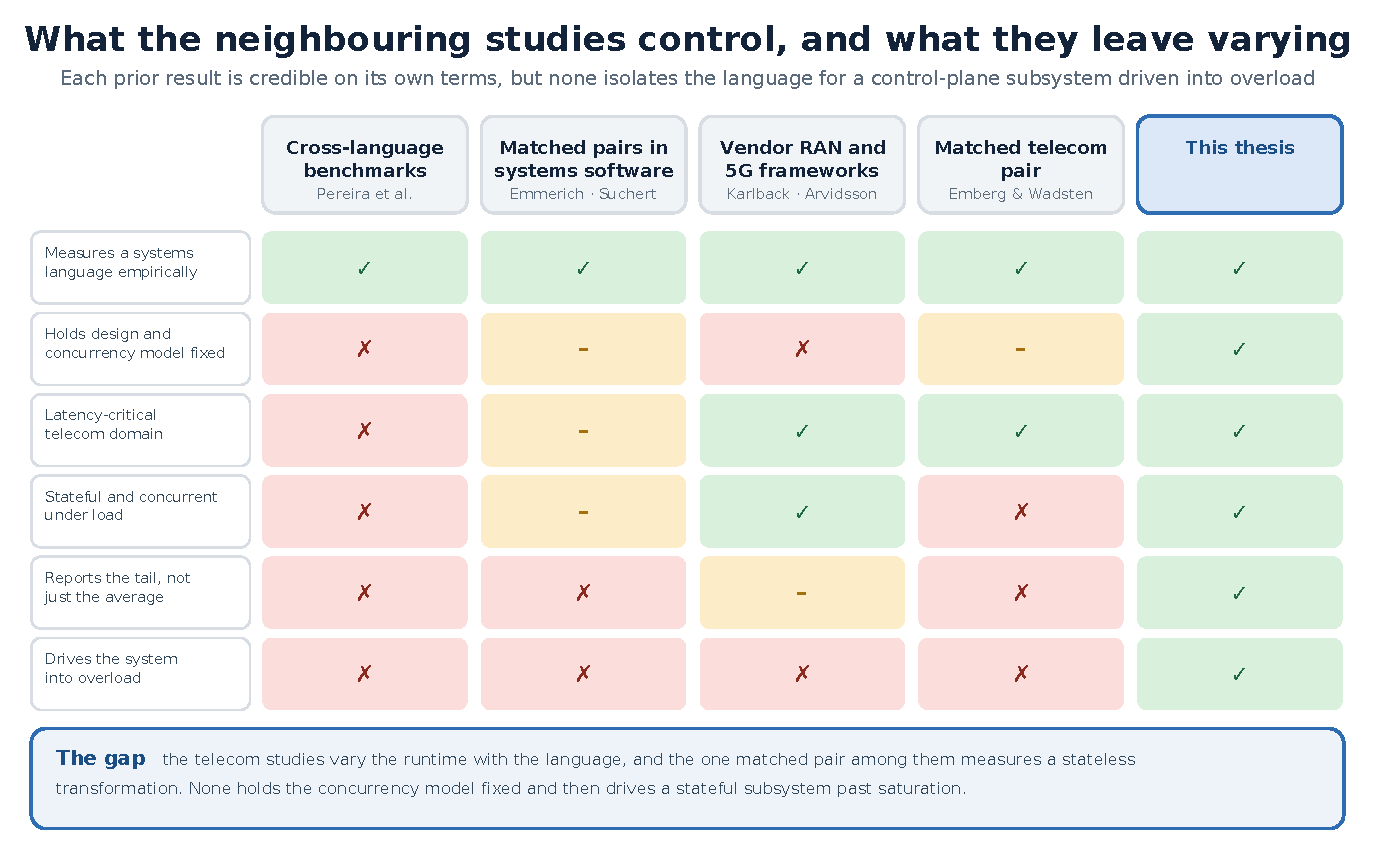
\includegraphics[width=0.78\linewidth]{diagrams/pdf/29_research_gap.pdf}
\caption[Các nghiên cứu lân cận kiểm soát gì, và để gì biến thiên]{Các nghiên cứu lân cận kiểm
soát gì, và để gì biến thiên. Mỗi hàng là một thuộc tính mà một câu trả lời có kiểm soát sẽ
cần, và mỗi cột là một nhóm nghiên cứu. Cột RAN nhà cung cấp là các luận văn Ericsson trừ
Emberg và Wadsten, những người có cột riêng vì họ giữ thiết kế sát hơn.\label{fig:gapmap}}
\end{figure}

Điều còn thiếu trong công trình trước là một phép thử trực tiếp, có kiểm soát, trên một phần
mặt điều khiển điển hình. Các câu hỏi mở như sau. Rust có giữ độ trễ đuôi khi tải quá lớn đối
với C++ hiện đại khi mô hình luồng, thao tác và bố cục dữ liệu được giữ cố định? Nó loại những
lớp lỗi nào, và phần còn lại bị bắt ở giai đoạn nào? Mô hình an toàn của nó tốn gì về thông
lượng và về CPU cùng bộ nhớ? Áp dụng từng bước tốn gì trên thực tế? Đóng khoảng trống này là
mục đích của bốn câu hỏi nghiên cứu. Chương tiếp theo neo chúng vào phần đang được nghiên cứu,
các lớp lỗi, và thời gian đang bị đe dọa. Nó cũng nêu phương pháp.
